\documentclass[11pt,a4paper,twoside,openright, openany]{book}
% Base packages ----------------------------------------------------------------
\usepackage{ragged2e}
\usepackage{verbatim}
\usepackage[T1]{fontenc}     % adds support for printing accented characters
\usepackage[utf8]{inputenc}  % adds support for inputting accented characters


\usepackage[square]{natbib}  %citation style
\bibliographystyle{apalike} 
\setcitestyle{aysep={:},yysep={;}}
%\let\cite=\citeauthor

\usepackage{hyperref}        % insert clickable hyperlinks
\usepackage{lastpage}        % reference last page (used to count numbered pages)


% Math packages ----------------------------------------------------------------
\usepackage{amsmath,amssymb,stmaryrd,mathtools,mathrsfs,bbm}  

% Other symbols 
\usepackage{textcomp} 
\usepackage{physics}
\usepackage{siunitx}    % si-units
\usepackage{gensymb}

% Figure packages --------------------------------------------------------------
\usepackage[dvipsnames, table, xcdraw]{xcolor}    % font colouring functionality
\usepackage{pgfplots}
\usepackage{graphicx}              % handling of images
\usepackage{booktabs}              % improved tables
\usepackage{array}                 % setting rowheight

\usepackage{algorithm}             % algorithm floats
\usepackage[noend]{algpseudocode}  % pseudocode listings
\usepackage{listings}              % source code listings
\usepackage{enumerate}
\usepackage{enumitem}
\usepackage{colortbl}              % table color
\usepackage{multirow}
\usepackage{makecell}
% Styling packages -------------------------------------------------------------

\usepackage{microtype}             % improve full justification and font kerning
\usepackage{emptypage}             % suppress page numbering on empty pages
\usepackage{fancyhdr}              % easy customisation of headers and footers
\usepackage{titlesec}              % easy customisation of section titles
\usepackage[margin=3cm]{geometry}  % adjust page margins
\usepackage[toc,page]{appendix}    % improved appendix control
\usepackage{framed}                % environments package
\usepackage[framed,amsmath,thmmarks]{ntheorem} % environments package
\usepackage{stfloats}              % linking tables to bottom of page
\usepackage{etoolbox}              % align removal spacing
\usepackage[parfill]{parskip}      % removes indent on new line

% Font packages ----------------------------------------------------------------
\usepackage{lmodern}  % improved default font
%todo
\usepackage[
%  disable,                  % turn off todonotes
  colorinlistoftodos,        % enable a coloured square in the list of todos
  textwidth=\marginparwidth, % set the width of the todonotes
  textsize=scriptsize,       % size of the text in the todonotes
  ]{todonotes}

% Theorem environments -----------------------------------------------------------

% \theoremheaderfont{\normalfont\bfseries}
% \theorembodyfont{\normalfont}
% \theoremstyle{break}
% \def\theoremframecommand{{\color{ForestGreen!50}\vrule width 5pt \hspace{5pt}}}
% \newshadedtheorem{lemma}{Lemma}[chapter]

% \def\theoremframecommand{{\color{red!50}\vrule width 5pt \hspace{5pt}}}
% \newshadedtheorem{example}{Example}[chapter]

% \def\theoremframecommand{{\color{ForestGreen!80}\vrule width 5pt \hspace{5pt}}}
% \newshadedtheorem{corollary}{Corollary}[chapter]

% \def\theoremframecommand{{\color{MidnightBlue!100}\vrule width 5pt \hspace{5pt}}}
% \newshadedtheorem{definition}{Definition}[chapter]

% \def\theoremframecommand{{\color{RoyalBlue!70}\vrule width 5pt \hspace{5pt}}}
% \newshadedtheorem{theorem}{Theorem}[chapter]

% \def\theoremframecommand{{\color{RoyalBlue!30}\vrule width 5pt \hspace{5pt}}}
% \newshadedtheorem{proof}{Proof}[chapter]

% \renewcommand\qedsymbol{$\blacksquare$}           % use black square as QED

% \def\exampleautorefname{Example}

% \def\definitionautorefname{Definition}

% Redefinition of theoremstyle break used for defined environments

\makeatletter
\renewtheoremstyle{break}%
  {\item[\rlap{\vbox{\hbox{\hskip\labelsep \theorem@headerfont
          ##1\ ##2\theorem@separator}\hbox{\strut}}}]}%
  {\item[\rlap{\vbox{\hbox{\hskip\labelsep \theorem@headerfont
%          ##1\ ##2\ (##3)\theorem@separator}\hbox{\strut}}}]}% DELETED
           ##1\ ##2:\ ##3\theorem@separator}\hbox{\strut}}}]}% NEW
\makeatother



\definecolor{defcolor}{rgb}{0.36, 0.54, 0.66}

\definecolor{lemmacolor}{rgb}{0.66, 0.89, 0.86}

\definecolor{corollarycolor}{rgb}{0.13, 0.67, 0.8}

\definecolor{thmcolor}{rgb}{0.29, 0.70, 0.70}

\definecolor{axiomcolor}{rgb}{1, 0.84, 0}
%%%%%%%%%%%%%%%%%%%%%%%%%%%%%%%%%%%%%%%%%%%%%%%%
% A theorem environment
%%%%%%%%%%%%%%%%%%%%%%%%%%%%%%%%%%%%%%%%%%%%%%%%
\theoremheaderfont{\normalfont\bfseries}
\theorembodyfont{\normalfont}
\theoremsymbol{}
\theoremstyle{break}
\def\theoremframecommand{{\color{thmcolor}\vrule width 3pt \hspace{5pt}}}
\newshadedtheorem{theorem}{Theorem}[chapter]
\newenvironment{theo}[1][\unskip]{%
		\begin{theorem}[#1]
}{%
		\end{theorem}
}
\def\theoremautorefname{Theorem}
%%%%%%%%%%%%%%%%%%%%%%%%%%%%%%%%%%%%%%%%%%%%%%%%
% A Proof environment
%%%%%%%%%%%%%%%%%%%%%%%%%%%%%%%%%%%%%%%%%%%%%%%%

\theoremheaderfont{\normalfont\itshape\bfseries}
\theorembodyfont{\normalfont}
\theoremsymbol{\rule{1ex}{1ex}}
\theoremstyle{break}
\newtheorem*{proof}{Proof}[theorem]
\newenvironment{pro}[1][\unskip]{%
		\begin{proof}[#1]
}{%
        
		\end{proof}
}
\def\proofautorefname{Proof}

%%%%%%%%%%%%%%%%%%%%%%%%%%%%%%%%%%%%%%%%%%%%%%%%
% A Definition environment
%%%%%%%%%%%%%%%%%%%%%%%%%%%%%%%%%%%%%%%%%%%%%%%%
\theoremheaderfont{\normalfont\bfseries}
\theorembodyfont{\normalfont}
\theoremsymbol{}
\theoremstyle{break}
\def\theoremframecommand{{\color{defcolor}\vrule width 3pt 
\hspace{5pt}}}
\newshadedtheorem{definition}[theorem]{Definition}
\newenvironment{defi}[1][\unskip]{%
		\begin{defintion}[#1]
}{%
		\end{definition}
}
\def\definitionautorefname{Definition}

%%%%%%%%%%%%%%%%%%%%%%%%%%%%%%%%%%%%%%%%%%%%%%%%
% An axiom environment
%%%%%%%%%%%%%%%%%%%%%%%%%%%%%%%%%%%%%%%%%%%%%%%%
\theoremheaderfont{\normalfont\bfseries}
\theorembodyfont{\normalfont}
\theoremsymbol{}
\theoremstyle{break}
\def\theoremframecommand{{\color{axiomcolor}\vrule width 3pt \hspace{5pt}}}
\newshadedtheorem{axiom}[theorem]{Axiom}
\newenvironment{axi}[1][\unskip]{%
		\begin{axiom}[#1]
}{%
		\end{axiom}
}
\def\axiomautorefname{Axiom}

%%%%%%%%%%%%%%%%%%%%%%%%%%%%%%%%%%%%%%%%%%%%%%%%
% A Lemma environment
%%%%%%%%%%%%%%%%%%%%%%%%%%%%%%%%%%%%%%%%%%%%%%%%
\theoremheaderfont{\normalfont\bfseries}
\theorembodyfont{\normalfont}
\theoremsymbol{}
\theoremstyle{break}
\def\theoremframecommand{{\color{lemmacolor}\vrule width 3pt \hspace{5pt}}}
\newshadedtheorem{lemma}[theorem]{Lemma}
\newenvironment{lemm}[1][\unskip]{%
		\begin{lemma}[#1]
}{%
		\end{lemma}
}
\def\lemmaautorefname{Lemma}

%%%%%%%%%%%%%%%%%%%%%%%%%%%%%%%%%%%%%%%%%%%%%%%%
% A Corollary environment
%%%%%%%%%%%%%%%%%%%%%%%%%%%%%%%%%%%%%%%%%%%%%%%%
\theoremheaderfont{\normalfont\bfseries}
\theorembodyfont{\normalfont}
\theoremsymbol{}
\theoremstyle{break}
\def\theoremframecommand{{\color{corollarycolor}\vrule width 3pt \hspace{5pt}}}
\newshadedtheorem{corollary}[theorem]{Corollary}
\newenvironment{corol}[1][\unskip]{%
		\begin{corollary}[#1]
}{%
		\end{corollary}
}
\def\corollaryautorefname{Corollary}
%%%%%%%%%%%%%%%%%%%%%%%%%%%%%%%%%%%%%%%%%%%%%%%%
% An example environment
%%%%%%%%%%%%%%%%%%%%%%%%%%%%%%%%%%%%%%%%%%%%%%%%
\theoremheaderfont{\normalfont\bfseries}
\theorembodyfont{\normalfont}
\theoremsymbol{}
\theoremstyle{break}
\theoremprework{\bigskip\hrule}
\theorempostwork{\hrule\bigskip}
\newtheorem{example}[theorem]{Example}
\newenvironment{exa}[1][\unskip]{
\begin{example}[#1]
}{
\end{example}
}
\def\exampleautorefname{Example}

% Sets --------------------------------------------------------------------------
\newcommand{\N}{\mathbb{N}}  % natural numbers
\newcommand{\Z}{\mathbb{Z}}  % integers
\newcommand{\Q}{\mathbb{Q}}  % rational numbers
\newcommand{\R}{\mathbb{R}}  % real numbers
\newcommand{\C}{\mathbb{C}}  % complex numbers
\newcommand{\I}{\mathbb{I}}




\let\cite=\citep
\renewcommand{\exp}[1]{e^{#1}}


% Colours
\definecolor{aaublue}{RGB}{33,26,82}
\usepackage[table]{xcolor}



% Headers and footers -----------------------------------------------------------
\fancyhead{}                      % clear default header fields
\setlength{\headheight}{14pt}
\fancyhead[LE,RO]{\projectgroup}  % left on even, right on odd
\fancyhead[RE]{\leftmark}         % chapter name
\fancyhead[LO]{\rightmark}        % sections name
\fancyfoot{}                      % clear default footer fields
\fancyfoot[CE,CO]{\thepage}       % centered page numbers
\pagestyle{fancy}                 % activate fancy style


% Chapter titles ----------------------------------------------------------------
% http://mirrors.dotsrc.org/ctan/macros/latex/contrib/titlesec/titlesec.pdf
\titleformat
{\chapter}
[hang]
{\Huge\bfseries}
{\thechapter\enspace{|}\enspace}
{0pt}
{\Huge\bfseries}




\numberwithin{equation}{chapter}  % resets the counter of equation number each time a new \section is used

\usepackage{subcaption}
\usepackage{caption}
\usepackage{listings}
\usepackage{comment}
\usepackage{advdate}
\usepackage{dcolumn}
\usepackage{amsfonts}

\captionsetup[figure]{font={it}}
\captionsetup[table]{font={it}}
% table
\renewcommand{\arraystretch}{1.5}

%include bibliography in the table of content
\usepackage[nottoc]{tocbibind}


% Matrix v_line
\makeatletter
\renewcommand*\env@matrix[1][*\c@MaxMatrixCols c]{%
   \hskip -\arraycolsep
   \let\@ifnextchar\new@ifnextchar
   \array{#1}}
\makeatother
% Arrows for text 
%\usetikzlibrary{positioning, arrows.meta}
\tikzset{%
    myarrow/.style = {-Stealth, shorten >=5pt}
}
\usetikzlibrary{shapes,shadows,arrows,positioning,graphs,shapes.geometric,arrows.meta}
\usetikzlibrary{calc,intersections,through,hobby}
\usetikzlibrary{matrix}
\tikzset{point/.style={circle,inner sep=0pt,minimum size=3pt,fill=red}}
\newcommand{\mypoint}[2]{\tikz[remember picture]{\node[inner sep=0, anchor=base](#1){$#2$};}}
%Fancy circles.
\newcommand*\circled[1]{\tikz[baseline=(char.base)]{
            \node[shape=circle,draw,inner sep=2pt] (char) {#1};}}
%pagebreak align
\allowdisplaybreaks

%For pseudo code
\usepackage{algorithm,algpseudocode,float}
\usepackage{lipsum}
\usepackage[noend]{algpseudocode}
\makeatletter
\newenvironment{breakablealgorithm}
  {% \begin{breakablealgorithm}
   \begin{center}
     \refstepcounter{algorithm}% New algorithm
     \hrule height.8pt depth0pt \kern2pt% \@fs@pre for \@fs@ruled
     \renewcommand{\caption}[2][\relax]{% Make a new \caption
       {\raggedright\textbf{\ALG@name~\thealgorithm} ##2\par}%
       \ifx\relax##1\relax % #1 is \relax
         \addcontentsline{loa}{algorithm}{\protect\numberline{\thealgorithm}##2}%
       \else % #1 is not \relax
         \addcontentsline{loa}{algorithm}{\protect\numberline{\thealgorithm}##1}%
       \fi
       \kern2pt\hrule\kern2pt
     }
  }{% \end{breakablealgorithm}
     \kern2pt\hrule\relax% \@fs@post for \@fs@ruled
   \end{center}
  }
\makeatother

\makeatletter
\def\BState{\State\hskip-\ALG@thistlm}
\makeatother

\usepackage{cleveref}
\usepackage[american]{circuitikz}

\renewcommand{\b}[1]{%
  \ensuremath{\left[#1\right]}%
}

\newcommand{\p}[1]{%
  \ensuremath{\left(#1\right)}%
}

\newcommand{\diag}[1]{%
  \ensuremath{\text{diag}\left(#1\right)}%
}

\newcommand{\floor}[1]{%
  \ensuremath{\left\lfloor #1 \right\rfloor}%
}

\newcommand{\sigm}{%
  \ensuremath{\Sigma^{-1}}%
}

\newcommand{\sigtilde}{%
  \ensuremath{\Tilde{\Sigma}}%
}
\renewcommand{\d}{%
  \ensuremath{\underline{d}}%
}
\renewcommand{\mathbf}[1]{%
  \ensuremath{\boldsymbol{#1}}%
}
\newcommand{\D}{%
  \ensuremath{\underline{D}}%
}
\newcommand{\x}{%
  \ensuremath{\underline{x}}%
}


\newcommand{\ls}{%
  \ensuremath{\limsup_{n\rightarrow \infty}}%
}

\renewcommand{\part}[2]{%
  \ensuremath{\frac{\partial #1}{\partial #2}}%
}

\newcommand{\mpart}[2]{%
  \frac{\partial #1}{\partial #2}%
}




\usepackage{stackengine}
\def\defeq{\mathrel{\ensurestackMath{\stackon[2pt]{=}{\scriptstyle\Delta}}}}

\newcommand\scalemath[2]{\scalebox{#1}{\mbox{\ensuremath{\displaystyle #2}}}}

\usepackage{tikz-3dplot}
\def\projecttitle       {Self Supervised Learning for Noise-Robust Key Word Spotting. }
\def\projectsubtitle    {}
\def\projectperiod      {fall-semester 2023}
\def\projectdegree      {Mathematics-Technology}
\def\projectsemester    {9th Semester}
\def\projectsupervisors {Zheng-Hua Tan \\ Holder Severin Bovbjerg \\ Christophe Biscio}
\def\projectgroup       {jmark18@student.aau.dk}
\def\projectauthors     {
Jacob Mørk
}

%  A simple AAU report template.
%  2013-03-06 v. 1.0.0
%  Copyright 2010-2013 by Jesper Kjær Nielsen <jkn@es.aau.dk>
%
%  This is free software: you can redistribute it and/or modify
%  it under the terms of the GNU General Public License as published by
%  the Free Software Foundation, either version 3 of the License, or
%  (at your option) any later version.
%
%  This is distributed in the hope that it will be useful,
%  but WITHOUT ANY WARRANTY; without even the implied warranty of
%  MERCHANTABILITY or FITNESS FOR A PARTICULAR PURPOSE.  See the
%  GNU General Public License for more details.
%
%  You can find the GNU General Public License at <http://www.gnu.org/licenses/>.
%
%
%
% see, e.g., http://en.wikibooks.org/wiki/LaTeX/Customizing_LaTeX#New_commands
% for more information on how to create macros

%%%%%%%%%%%%%%%%%%%%%%%%%%%%%%%%%%%%%%%%%%%%%%%%
% Macros for the titlepage
%%%%%%%%%%%%%%%%%%%%%%%%%%%%%%%%%%%%%%%%%%%%%%%%
%Creates the aau titlepage
\newcommand{\aautitlepage}[3]{%
  {
    %set up various length
    \ifx\titlepageleftcolumnwidth\undefined
      \newlength{\titlepageleftcolumnwidth}
      \newlength{\titlepagerightcolumnwidth}
    \fi
    \setlength{\titlepageleftcolumnwidth}{0.5\textwidth-\tabcolsep}
    \setlength{\titlepagerightcolumnwidth}{\textwidth-2\tabcolsep-\titlepageleftcolumnwidth}
    %create title page
    \thispagestyle{empty}
    \noindent%
    \begin{tabular}{@{}ll@{}}
      \parbox{\titlepageleftcolumnwidth}{
        
\includegraphics[width=\titlepageleftcolumnwidth]{incl/main/aau-report-badge.pdf}
      } &
      \parbox{\titlepagerightcolumnwidth}{\raggedleft\sf\small
        #2
      }\bigskip\\
       #1 &
      \parbox[t]{\titlepagerightcolumnwidth}{%
      \textbf{Abstract:}\bigskip\par
        \fbox{\parbox{\titlepagerightcolumnwidth-2\fboxsep-2\fboxrule}{%
          #3
        }}
      }\\
    \end{tabular}
    \vfill
    \noindent{\footnotesize\emph{The content of this report is freely available, but publication (with reference) may only be pursued due to agreement with the authors.}}
    \clearpage
  }
}

%Create english project info
\newcommand{\englishprojectinfo}[8]{%
  \parbox[t]{\titlepageleftcolumnwidth}{
    \textbf{Title:}\\ #1\bigskip\par
    \textbf{Theme:}\\ #2\bigskip\par
    \textbf{Project Period:}\\ #3\bigskip\par
    \textbf{Project Group:}\\ #4\bigskip\par
    \textbf{Authors:}\\ #5\bigskip\par
    \textbf{Supervisors:}\\ #6\bigskip\par
    %\textbf{Copies:} #7\bigskip\par
    \textbf{Number of Pages:} \pageref{lastofmain}\bigskip\par
    \textbf{Date of Completion:}\\ #8
  }
}

%Create danish project info
\newcommand{\danishprojectinfo}[8]{%
  \parbox[t]{\titlepageleftcolumnwidth}{
    \textbf{Titel:}\\ #1\bigskip\par
    \textbf{Tema:}\\ #2\bigskip\par
    \textbf{Projektperiode:}\\ #3\bigskip\par
    \textbf{Projektgruppe:}\\ #4\bigskip\par
    \textbf{Forfattere):}\\ #5\bigskip\par
    \textbf{Vejledere:}\\ #6\bigskip\par
    %\textbf{Antal kopier:} #7\bigskip\par
    \textbf{Antal sider:}  \pageref{LastPage} \bigskip\par
    \textbf{Afleveringsdato:}\\ #8
  }
}

\ExplSyntaxOn
\NewDocumentCommand{\rvect}{m}
 {
  \seq_set_split:Nnn \l_tmpa_seq { , } { #1 }
  \begin{bmatrix}
  \seq_use:Nn \l_tmpa_seq { & }
  \end{bmatrix}
 }
\ExplSyntaxOff

% Indsæt python kode
\definecolor{codegreen}{rgb}{0,0.6,0}
\definecolor{codegray}{rgb}{0.5,0.5,0.5}
\definecolor{codepurple}{rgb}{0.58,0,0.82}
\definecolor{backcolour}{rgb}{0.95,0.95,0.92}

\lstdefinestyle{mystyle}{
    backgroundcolor=\color{backcolour},   
    commentstyle=\color{codegreen},
    keywordstyle=\color{magenta},
    numberstyle=\tiny\color{codegray},
    stringstyle=\color{codepurple},
    basicstyle=\ttfamily\footnotesize,
    breakatwhitespace=false,         
    breaklines=true,                 
    captionpos=b,                    
    keepspaces=true,                 
    numbers=left,                    
    numbersep=5pt,                  
    showspaces=false,                
    showstringspaces=false,
    showtabs=false,                  
    tabsize=2
}
\lstset{style=mystyle}

\newcommand\textline[2][t]{%
  \parbox[#1]{\textwidth}{\raggedleft{#2}}%
}
\newcommand{\DFTarrow}{\ensuremath{\,
\tikz{\coordinate(c)(0,0);\node[yshift=2pt,at=(c)](DFT){\small{$\mathcal{DFT}$}};\draw[<->, draw=black]([xshift=-12pt,yshift=-5pt]c)--([xshift=12pt,yshift=-5pt]c);} 
}\,}
\newcommand{\Cov}{\Sigma}
\newcommand{\Var}{\text{Var}}
\newcommand{\E}{\text{E}}
% \newcommand*{\defeq}{\stackrel{\blacktriangle}{=}}


\begin{document}
%\pagestyle{empty}
\cleardoublepage
\frontmatter\pagenumbering{roman}
% LaTex template, example front page
% ------------------------------------------------------------------------------

\begin{titlepage}
  \centering

  \vspace{2cm}

  % Title
  {\huge\bfseries\projecttitle}
  
  %\vspace{0.5cm}
  
  %{\Large\bfseries\sffamily\projectsubtitle}
    
  \vspace{2cm}

  % Figur
  
\includegraphics[width =0.8\textwidth]{incl/main/aau-report-badge.pdf}
  \vspace{1cm}
  
  \textsc{\LARGE P9 Project}\\
  \textsc{\Large Mathematical Engineering}


  \vspace{3cm}


  % Authors and supervisors
  \begin{minipage}[t]{0.4\textwidth}
    \begin{flushleft}
      \large
      \emph{Authors:}\\
      \projectauthors
    \end{flushleft}
  \end{minipage}
  \begin{minipage}[t]{0.4\textwidth}
    \begin{flushright}
      \large
      \emph{Supervisor:}\\
      \projectsupervisors
    \end{flushright}
  \end{minipage}

  \vfill

  {\large\today}
\end{titlepage}
\thispagestyle{empty}
{\small
\strut\vfill % push the content to the bottom of the page
\noindent Copyright \copyright{} Aalborg University 2023\par
\vspace{0.2cm}
\noindent Written with pdf\LaTeX.}
\clearpage
% LaTeX template, example title page
% ------------------------------------------------------------------------------
% The title page is generated by the command \aautitlepage, which is defined in
% macros.tex


\pdfbookmark[0]{Title page}{label:titlepage_en}
\aautitlepage{%
  \englishprojectinfo{
    \projecttitle  % project title
  }{%
    \projectsubtitle  % project theme
  }{%
    \projectperiod  % project period
  }{%
    \projectgroup  % project group
  }{
    % list of group members
    \projectauthors
  }{%
    % list of supervisors
    \projectsupervisors
  }{%
    1  % number of printed copies
  }{%
    \today  % date of completion
  }%
}{%
  % Department and address
  \textbf{Department of Mathematical Sciences}\\
  Skjernvej 4A\\
  Aalborg University\\
  \href{http://www.math.aau.dk}{http://www.math.aau.dk}
}{
  \input{incl/misc/abstract}
}
\begin{table}[b]
	\centering
		% \begin{tabular}{c c c}
		% 	\underline{\phantom{mmmmmmmmmmmmmm}} & \underline{\phantom{mmmmmmmmmmmmmm}} \\
		% 	Anders Lauridsen		& Jacob Mørk \\
		% 	&&\\
		% 	&&\\
		% 	&&\\
		% \end{tabular}
		\begin{tabular}{c c c}
			\underline{\phantom{mmmmmmmmmmmmmm}} \\
			Jacob Mørk	
		\end{tabular}
\end{table}

\chapter*{Preface}
This project has been written in the period from September 1st, 2023 to December 25th, 2023 by one Mathematical Engineering students at Aalborg University the third semester of the master's. I would like to thank supervisors Zheng-Hua Tan and Christophe Biscio for their support throughout the project period. I would also like to thank Holger Severin Bovbjerg for the additional help throughout the duration of the project.
\\
In this project, it is assumed that the reader has an understanding of the subjects presented during study for the bachelor's and master's degrees in Mathematical Engineering from Aalborg University.\\ \\
\textline[t]{Aalborg University, \today}
%\chapter*{Nomenclature}


\tableofcontents

\mainmatter\pagenumbering{arabic}

% Input chapters
    \chapter{Introduction} \label{ch:intro}
        Today keyword spotting (KWS) is implemented in various systems like voice assistants. For these systems to achieve satisfying performance the models typically rely on a large amount of labeled data. This is limiting these application to situations where only this kind of data is available. To accommodate for this problem [Holgers article] has been looking into using self supervised learning (SSL). 

Self supervised learning (SSL) have existed for a while, and while it has been the same idea driving the SSL in different fields, the implementations has differed [source: Data2vec article, abstract]. Therefor [Data2vec article] has introduced, what they call data2vec, which is a \textit{framework that uses the same learning method for either speech, NLP, or computer vision}.

Since most systems using KWS are implemented places with some or more background noise. If you use speech commands on your phone the background noise could be anything from a bus stopping to people speaking.

In today's society, it is almost a given that new technology have some level of voice assistants, whether it is simple voice commands or integrated voice assistants, like Apple's Siri or Google's Assistant, keyword spotting is a part of it. For the voice assistants, there is an activating keyword. Using a keyword, it is possible to avoid running a more computational expensive automatic speech recognition (ASR) when it is not needed. Keyword spotting (KWS) also has many other applications, such as speech data mining, audio indexing, and phone call routing [KWS overview]. 
    
    \chapter{Keyword Spotting}
        Keyword spotting (KWS) has developed a lot over the years with one of the earliest approaches being based on the use of large-vocabulary continuos speech recognition (LVCSR) systems. An advantage to LVCSR-based KWS is its flexibility to deal with changing/non-predefined keywords. However, a big weakness to the LVCSR-based KWS is that it requires a large amount of computational resources, which can result in latency. This is an import factor when working with smaller online devices such as smartphones and smartwatches. A lighter alternative to LVCSR-based KWS is the keyword/filler hidden Markov model (HMM) approach. This approach trains a keyword HMM and a filler HMM to model keywords and non-keywords audio segments, respectively. Viterbi decoding is applied at runtime to find the optimal path in the decoding graph. Viterbi decoding can end up being computational demanding, depending on the topology of the HMM. The KWS system is then triggered whenever the likelihood ratio of the keyword model versus filler model is larger than a set threshold \cite{lopez2021deep}. 

Deep neural networks (DNN) have become very popular and are being used to develop new KWS systems. These systems are referred to as deep KWS systems and have become the new state of the art in KWS. Deep KWS systems do not need any complicated search algorithms like viterbi decoding, and they come with a huge improvement over the keyword/filler HMM approach in the case of low computational complexity \cite{lopez2021deep}. In general, deep KWS systems consist of three steps: speech features extraction, DNN acoustic model, and posterior handling, which is illustrated in \Cref{fig:deep_kws_system}.

\begin{figure}[h]
    \centering
    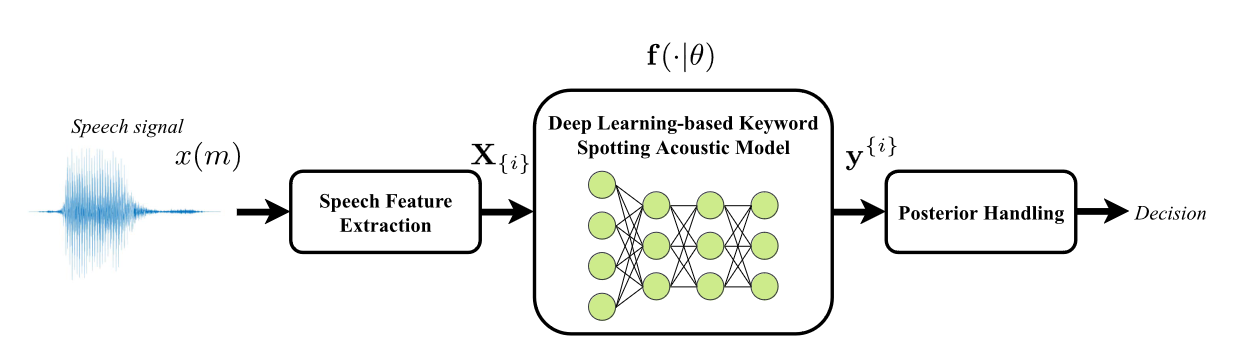
\includegraphics[width=\textwidth]{incl/img/kws/deep_kws_system.png}
    \caption{ Deep KWS system, from \cite{lopez2021deep}}
    \label{fig:deep_kws_system}
\end{figure}

\section{Speech Feature Extraction}
The speech feature extractor converts a speech signal, \(x(m)\), to a more compact representation of the speech. The speech features are often represented as a two dimensional matrix,
\begin{align}
    \textbf{X} = (\textbf{x}_0, \dots, \textbf{x}_{T-1}) \in \R^{K\times T},
\end{align}
where \(T\) is the amount of feature vectors, and \(K\) is the size of each feature vector. The amount of feature vectors depends on the length of the speech signal \cite{lopez2021deep}. 

Some of the popular speech features are the Mel-scale-related features. These could be the log-Mel spectral coefficients and Mel-frequency cepstral coefficients (MFCCs) \cite{lopez2021deep}. The common way to extract the log-Mel spectral and the MFCC features is shown on \Cref{fig:MFCC}. On the figure, it can be seen that to obtain the MFCC features you first have to get the log-Mel spectrogram coefficients, and then apply the discrete cosine transform to it. To stabilize and speed up the training of the DNN acoustic model, the features are normalized to a mean of zero and a standard deviation of one. This will also make the model more generalized \cite{lopez2021deep}. 

\begin{figure}[h]
    \centering
    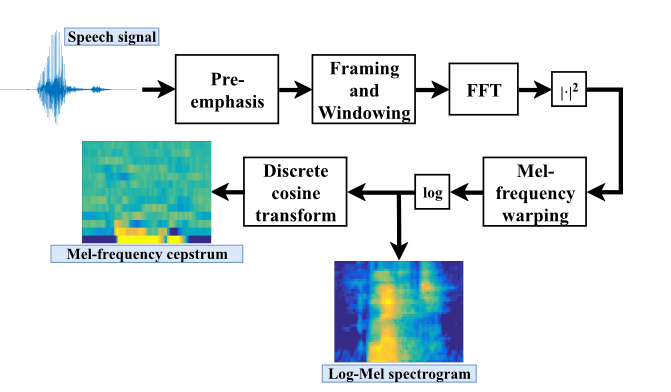
\includegraphics[width=\textwidth]{incl/img/kws/MFCC.png}
    \caption{ Classical pipeline for extracting log-Mel spectral and
    Mel-frequency cepstral speech features using the fast Fourier transform
    (FFT) \cite{lopez2021deep}}
    \label{fig:MFCC}
\end{figure}


\section{DNN KWS acoustic model}
The output of the speech feature extraction \(\textbf{X}\) is fed to the DNN acoustic model, which then outputs a sequence of probabilities, one for each keyword and non-keyword class. The way the acoustic model go through \(\textbf{X}\) is by taking a smaller section at a time, each section given as
\begin{align}
    \textbf{X}_{\{i\}} = \qty(\textbf{x}_{is-P}, \dots, \textbf{x}_{is}, \dots, \textbf{x}_{is+F}) \in \R^{K\times (P+F+1)},
\end{align} 
where \(i = \lceil \frac{P}{s} \rceil, \dots, \lfloor \frac{T-1-F}{s} \rfloor\) is a segment, \(s\) represents the time shift i.e., the overlap, \(P\) is the number of past frames, and \(F\) the number of future frames. Two examples of consecutive sections are illustrated on \Cref{fig:acoustic_model}. 

Denoting the DNN acoustic model as 
\begin{align}
    \textbf{f}\qty(\cdot|\theta): \R^{K\times (P+F+1)} \rightarrow I^N, 
\end{align}
where \(\theta\) is the input of the model, \(I = [0,1]\), and \(N\) the number of classes, we get the output probabilities, \(\textbf{y}^{\{i\}}\), of the model, given a segment \(\textbf{X}_{\{i\}}\),
\begin{align}
    \textbf{y}_n^{\{i\}} = \textbf{f}_n\qty(\textbf{X}_{\{i\}}|\theta), \quad n = 1, \dots, N,
\end{align}
where \(n\) denotes the \(n\)'th element of a vector. Denoting \(C_n\) as the \(n\)'th class we get that \(\textbf{y}_n^{\{i\}} = P(C_n|\textbf{X}_{\{i\}}, \theta)\) is the probability of \(\textbf{X}_{\{i\}}\) belonging to \(C_n\). To ensure that \(\textbf{y}_n^{\{i\}}\) is a probability, i.e., 
\begin{align}
    \sum_{n=1}^N \textbf{y}_n^{\{i\}} = 1 \quad \forall \ i,
\end{align}
a softmax activation function \cite{rothman2020artificial} is commonly used on the last layer \cite{lopez2021deep}.

\begin{figure}[h]
    \centering
    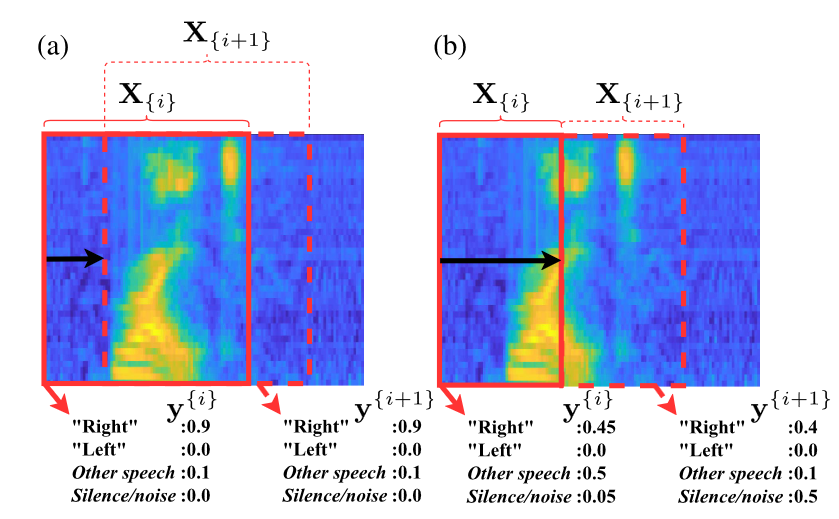
\includegraphics[width=\textwidth]{incl/img/kws/acoustic_model.png}
    \caption{Example of the processing of two consecutive feature segments \(\textbf{X}_{\{i\}}\) and \(\textbf{X}_{\{i +1\}}\), from \(\textbf{X}\) comprising the keyword "right", by a DNN acoustic model: (a) when using an overlapping segmentation window, and (b) when using a smaller, non-overlapping one \cite{lopez2021deep}. }
    \label{fig:acoustic_model}
\end{figure}

To pick which class a certain segment belongs to, one could just pick the class with highest probability, which could lead to different errors. Two cases where this approach will fail are shown in \Cref{fig:acoustic_model}, where an overlapping segment window is used on (a), and a smaller non-overlapping segment is used on (b). In the case of (a) the word "right" is found twice leading to a false positive detection and in the case of (b), "right" is not found a single time, leading to a false negative. This is one of the reasons why a good posterior handling is needed \cite{lopez2021deep}.

\subsection{Transformer Models}
The keyword transformer 

The KWT model is based on a vision transformer \cite{dosovitskiy2020image}, where the image is substituted with Mel-frequency cepstral coefficients (MFCC), which are explained in \Cref{ch:theory}, and have achieved state-of-the-art performance on the Google Speech Commands KWS benchmark.

\section{Posterior Handling}
To get a good final decision of class, the sequence of probabilities, \(\textbf{y}^{\{i\}}\), needs to be processed. There are two main modes when applying posterior handling: non-streaming and streaming modes.

\textbf{Non-streaming mode} is the simpler of the two, it is a standard multi-class classification of independent input segments. Since it only works on one segment, the segment needs to be long enough to contain a whole word – this could be around one second. \cite{lopez2021deep}. Posterior handling, in this mode, is the straight forward method of picking the class with the highest probability. This is not a very realistic method, because KWS in not a static task \cite{lopez2021deep}.

\textbf{Streaming mode} is, on the other hand, when the processing happens continuously, and normally in real-time \cite{lopez2021deep}. In this mode, the output sequence of probabilities from the acoustic model
\begin{align}
    \qty\{ \dots, \textbf{y}^{\{i-1\}}, \textbf{y}^{\{i\}}, \textbf{y}^{\{i+1\}}, \dots\},
\end{align}
is typically smoothened over time, classically a moving average is used. The smoothed probabilities, \(\bar{\textbf{y}}^{\{i\}}\), are often used to determine the keyword, or the lack of one. This is done either by comparing them with a sensitive threshold or by picking the class with the highest probability within a time sliding window. In the case of two consecutive segments covering the same keyword, a simple method is implemented, where all spotted keywords are ignored for a short period of time right after a keyword is spotted.



    \chapter{Self-Supervised Learning} \label{ch:theory}
        \section{Self-Supervised Learning}
Self-Supervised Learning (SSL) is, unlike supervised learning, learning information about some data without any labels. The way SSL is not unsupervised is by defining a learning objective based on the underlying structure of the data itself, this is called a pretext task.
In general this in done by predicting any unobserved or hidden part of the input data using only the observed or unhidden part of the input data. 
For natural langues processing (NLP) one way to do so is by hide words and try to predict the hidden words. a common way to do so is using masks. When using masks the objective is to predict the masked word from the surrounding words. This encourage the model to learn the relationships between different words, which then can be utilized in a range of downstream tasks. This could for example be translating text, summarizing, or generating text. 
In computer vision (CV) the same approach, predicting masked patches of an image or representation, have been used in models such as MAE and BYOL [KILDER]. Other approaches are also common in CV, for example using the objective of mapping two versions of the same image to the same representations.
Even though the idea of SSL is very similar across different domains, such as NLC, CV, or audio, their algorithms and objectives are very different. This is mainly because they were developed with a single domain in mind. A framework which is created with multiple domains in mind is data2vec.

\todo[inline]{Maybe add some from data2vec article into \\This is mainly from Meta Cookbook}

\section{Data2vec}
Data2vec is a framework which is created to get closer to one leaning method for all SSL problems. The version of data2vec which is used in this project has implemented a method which works on either speech, NLP, or CV. The method used combines masked prediction with the learning of latent target representations generalized by using multiple network layers as targets. This is done by having a student mode and a teacher mode. First the input data is masked and encoded to create a representation of the masked input. The unmasked input data is then encoded and parameterized as an exponential moving average to create the training targets. Now the learning objective is for the student to predict the target representations, given a partial view of the input. This is illustrated on \Cref{fig:data2vec_ilu}.

\begin{figure}
    \centering
    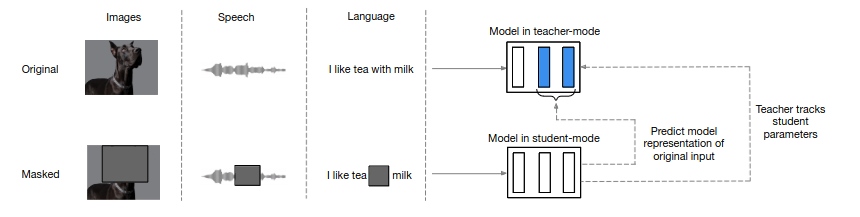
\includegraphics[width=\textwidth]{incl/img/data2vec/data2vec_ilu.png}
    \caption{An illustration of how data2vec works on different data types, using the same process. The model creates a representation of the original input data and then a masked version of the input.}
    \label{fig:data2vec_ilu}
\end{figure}

% To create the representations on the different data types models there are used encoders specified to the datatype.

The way the model is trained is to predict the representation of the unmasked sample, only knowing the encoding of the masked sample.

% Herfra, I dont know....
In the teacher mode the encoding is parameterized by an exponential moving average of the model parameters where the weights of the model in target-mode \(\Delta\) are
\begin{align}
    \Delta \leftarrow \tau \Delta + (1-\tau)\theta,
\end{align}
where \(\theta\) is the model parameters, and \(\tau\) is linearly increasing from \(\tau_0\) to \(\tau_e\) over the first \(\tau_n\) updates and are constant hereafter. This makes the teacher update more frequently in the beginning of the training when the model is more random and less frequently when good parameters have been learned.

The training targets are constructed from the last \(K\) blocks of parameters from the teacher network at the same time step as the student network. The training target at time step \(t\), for a network with \(L\) blocks in total, is then
\begin{align}
    y_t = \sum_{l=L-K+1}^L \hat{a}_t^l,
\end{align}
where \(\hat{a}_t^l\) is the normalized output of block \(l\) at time step \(t\). The normalizing helps the network not to collapse and layers with high norm to not dominate the target feature. For speech the normalizing used is instance normalizing \cite{ulyanov2016instance} without any learned parameters over the current input sample, this is because the neighboring representations are highly correlated due to small stride over the input data. Whereas for NLP and CV a parameter-less layer normalization \cite{ba2016layer} is used. 

    \chapter{Experiment} \label{ch:experiment}
        In this chapter the experiment will be outlined, whereafter the results of the experiment will be presented. The experiment includes five different models: two baseline, and three test models.

\section{Data}
The data used in this project is the Google Speech Commands V2 dataset \cite{warden2018speech}, which consists of \(105829\) one second recordings of \(35\) different keywords, outlined in \Cref{tab:google_words}. The dataset has been manipulated such that \(80\%\) of the training data are without labels. The \(80\%\) will be used to pretrain the models, and the remaining \(20\%\) will then be used to finetune the models and to train a baseline model. The final spilt of the recordings can be seen in \Cref{tab:data_split}

\begin{table}[ht]
    \centering
    \begin{tabular}{@{}lcccc@{}}
        \toprule
        Use    & Pretraining & \makecell{ finetuning/ \\ Baseline } & Validating & Testing \\ \midrule
        Recordings   & 67874  & 16969 & 9981 & 11005 \\ 
        \bottomrule
    \end{tabular}
    \caption{How the 105820 recordings are split}
    \label{tab:data_split}
\end{table}

Four different types of noise are used in the experiment, which can be put into two categories, one being stationary an another being non-stationary. The two types of noises in the stationary category are bus (BUS) and cafe (CAF), which have been used by \cite{barker2015third}. The other two types of noises are babble (BBL) and speech shaped noise (SSN), which were generated by \cite{kolboek2016speech}. The noises have been added to the keywords in \(7\) different SNR's: \(-10, \ -5, \ 0, \ 5, \ 10, \ 15, \ 20\). This yields \(28\) datasets, one for each noise with each SNR.
For each SNR two mixed data sets have been created, one is a \(50/50\) mixture of keywords with BUS and BBL noise. Another mixed dataset is a equal mixture of keywords with all types of noise.

\section{Model Setup}
The training and testing is using the same setup and models as in \cite{bovbjerg2023improving}. Here a keyword transformer (KWT) \cite{berg2021keyword}, with a added mean of the encodings of each time step, is used. 
%The KWT model is based on a vision transformer \cite{dosovitskiy2020image}, where the image is substituted with Mel-frequency cepstral coefficients (MFCC), which are explained in \Cref{ch:theory}, and have achieved state-of-the-art performance on the Google Speech Commands KWS benchmark.

Following \cite{bovbjerg2023improving}, three versions of the KWT is used. Varying the transformers amount of attention heads from one to three and the encoder dimension from \(64\) to \(192\) yields the three models: KWT-1, KWT-2, and KWT-3, with \(0.6\cdot 10^6\), \(2.4\cdot 10^6\), and \(5.4 \cdot 10^6\) parameters respectively \cite{bovbjerg2023improving}. 

In order to validate the noise-robustness of the SSL model two baseline models are trained. One being the baseline-supervised, which is a fully supervised model trained on the \(20\%\) labeled data. 
The second baseline model is a model pretrained and finetuned using noiseless data, this model is referred to as the baseline-Data2vec model. The three test models are all finetuned on the same data as the baseline-supervised is trained on and pretrained on different data. One is trained on noiseless data, and another is trained on noisy data, these are referred to as pretrained-noiseless and pretrained-noisy respectively. The last test model is trained by feeding to the student noisy data and the teacher with noiseless data, this model is referred to as the pretrained-both model. 

Training the five models three times, one with each KWT results in \(15\) models in total.


\subsection{Model Training}
Using the same setup as in \cite{bovbjerg2023improving} the finetuning and baseline-supervised model is trained for \(140\) epochs with a batch size of \(512\), using cross entropy as the learning objective. The weights are updated using the AdamW \cite{loshchilov2018fixing} optimizer with a learning rate of \(1 \cdot 10^ {-3}\) and a weight decay of \(0.1\), where the learning rate schedular used is a \(10\) epochs linear warmup followed by cosine annealing. Furthermore, doing the training of the model SpecAugment \cite{park2019specaugment} is randomly applied to mask blocks in both time and feature dimension \cite{bovbjerg2023improving}. 

For the pretraining the time domain masking strategy is the same as used in Wav2Vec \cite{}. Here a MFCC vector is picked with probability of \(0.65\) and the next \(10\) MFCC vectors are then replaced by a mask token embedding. The hyperparameters used are the same as the ones used in \cite{bovbjerg2023improving}, where most of the hyperparameters have been chosen according to the original Data2vec study \cite{baevski2022data2vec}, with a few changes due to different in data and hardware.

The models have been train using the implementation created by the author of \cite{bovbjerg2023improving}. 

\section{Test Setup}
The experiment consists of two tests. In the first test the same kind of noise as in the training (i.e., BUS and BBL) is added, but using only one SNR. The accuracy of the \(15\) models are then found for each SNR. The results of this test can be found in \Cref{subsec:test1}.

The second test is performed using the four noise types (i.e., BUS, BBL, CAF, and SSN). The results of this test can be found in \Cref{subsec:test2}.


%For these tests \(63\) models have been trained. A KWT-1, a KWT-2, and a KWT-3 model have been trained using both the baseline method, the pretraining on clean data, and pretraining on noisy data, for each SNR. The noise added to the training data is af \(50/50\) mix of CAF and BBL.

%The first test is testing the models on data where the same kind of noise as used in the training have been added, i.e., CAF and BBL. For the second test 
        \section{Results} \label{results}
In this section, the results of the test are presented. There are two levels to the test, one where the models are tested on keywords where the same kind of noise is applied, and one where more types of noise are added to the test set. 

\subsection{Testing on the Same Noise} \label{subsec:test1}
The different models are tested using a test set created of different sound files where the same kind of noise, as the model is trained on, is added. The results are presented in \Cref{tab:test_noise}, where a subtable for each noise level is presented. 

\begin{table}[ht]
    \centering
    \begin{tabular}{@{}llllll@{}}
        \multicolumn{6}{c}{\textbf{KWT-1}}\\
        \toprule
        % &  & & \multicolumn{3}{c}{Data2vec pretraining} \\ \cline{4-6}
        SNR    & \makecell{ Baseline - \\ Supervised } & \makecell{ Baseline - \\ Deta2vec } & \makecell{ Pretrained - \\ Noiseless } & \makecell{ Pretrained - \\ Noisy } & \makecell{ Pretrained - \\ Both } \\ \midrule
        -10  & 0.3460 & -- & 0.3784 & 0.3825 & -- \\
        -5   & -- & -- & -- & -- & -- \\
        0    & -- & -- & -- & -- & -- \\
        5    & -- & -- & -- & -- & -- \\
        10   & -- & -- & -- & -- & -- \\
        15   & -- & -- & -- & -- & -- \\
        20   & -- & -- & -- & -- & -- \\
        
        \bottomrule
    \end{tabular}
    \caption{KWT-1}
    \label{tab:KWT-1_snrmix_busxbbl}
\end{table}

\begin{table}[ht]
    \centering
    \begin{tabular}{@{}llllll@{}}
        \multicolumn{6}{c}{\textbf{KWT-2}}\\
        \toprule
        % &  & & \multicolumn{3}{c}{Data2vec pretraining} \\ \cline{4-6}
        SNR    & \makecell{ Baseline - \\ Supervised } & \makecell{ Baseline - \\ Deta2vec } & \makecell{ Pretrained - \\ Noiseless } & \makecell{ Pretrained - \\ Noisy } & \makecell{ Pretrained - \\ Both } \\ \midrule
        -10  & 0.3133 & -- & 0.3888 & 0.4052 & -- \\
        -5   & -- & -- & -- & -- & -- \\
        0    & -- & -- & -- & -- & -- \\
        5    & -- & -- & -- & -- & -- \\
        10   & -- & -- & -- & -- & -- \\
        15   & -- & -- & -- & -- & -- \\
        20   & -- & -- & -- & -- & -- \\
        
        \bottomrule
    \end{tabular}
    \caption{KWT-2}
    \label{tab:KWT-2_snrmix_busxbbl}
\end{table}

\begin{table}[ht]
    \centering
    \begin{tabular}{@{}llllll@{}}
        \multicolumn{6}{c}{\textbf{KWT-3}}\\
        \toprule
        % &  & & \multicolumn{3}{c}{Data2vec pretraining} \\ \cline{4-6}
        SNR    & \makecell{ Baseline - \\ Supervised } & \makecell{ Baseline - \\ Deta2vec } & \makecell{ Pretrained - \\ Noiseless } & \makecell{ Pretrained - \\ Noisy } & \makecell{ Pretrained - \\ Both } \\ \midrule
        -10  & 0.2970 & -- & 0.3602 & 0.3817 & -- \\
        -5   & -- & -- & -- & -- & -- \\
        0    & -- & -- & -- & -- & -- \\
        5    & -- & -- & -- & -- & -- \\
        10   & -- & -- & -- & -- & -- \\
        15   & -- & -- & -- & -- & -- \\
        20   & -- & -- & -- & -- & -- \\
        
        \bottomrule
    \end{tabular}
    \caption{KWT-3}
    \label{tab:KWT-3_snrmix_busxbbl}
\end{table}


\begin{table}[ht]
    \centering
    \begin{subtable}[ht]{0.45\textwidth}
        \centering
        \begin{tabular}{@{}llll@{}}
        \toprule
        & & \multicolumn{2}{c}{Data2vec pretraining} \\ \cline{3-4}
        snr-10    & \makecell{ Baseline - \\ Supervised } & \makecell{ Pretrained - \\ Noiseless } & \makecell{ Pretrained - \\ Noisy } \\ \midrule
        KWT-1    & 0.3460  & 0.3784 & 0.3825 \\
        KWT-2    & 0.3133  & 0.3888 & 0.4052 \\
        KWT-3    & 0.2970  & 0.3602 & 0.3817 \\
        \bottomrule
        \end{tabular}
        \caption{Snr -10}
    \end{subtable}
    \hfill
    \begin{subtable}[ht]{0.45\textwidth}
        \centering
        \begin{tabular}{@{}llll@{}}
        \toprule
        & & \multicolumn{2}{c}{Data2vec pretraining} \\ \cline{3-4}
        snr-5    & \makecell{ Baseline - \\ Supervised } & \makecell{ Pretrained - \\ Noiseless } & \makecell{ Pretrained - \\ Noisy } \\ \midrule
        KWT-1    & --  & -- & -- \\
        KWT-2    & --  & -- & -- \\
        KWT-3    & --  & -- & -- \\
        \bottomrule
        \end{tabular}
        \caption{Snr -5}
    \end{subtable}
     
     
    \bigskip


    \begin{subtable}[ht]{0.45\textwidth}
        \centering
        \begin{tabular}{@{}llll@{}}
        \toprule
        & & \multicolumn{2}{c}{Data2vec pretraining} \\ \cline{3-4}
        snr0    & \makecell{ Baseline - \\ Supervised } & non-noise & \makecell{ Pretrained - \\ Noisy } \\ \midrule
        KWT-1    & --  & -- & 0.698 \\
        KWT-2    & --  & -- & -- \\
        KWT-3    & --  & -- & -- \\
        \bottomrule
        \end{tabular}
        \caption{Snr 0}
    \end{subtable}
    \hfill
    \begin{subtable}[ht]{0.45\textwidth}
        \centering
        \begin{tabular}{@{}llll@{}}
        \toprule
        & & \multicolumn{2}{c}{Data2vec pretraining} \\ \cline{3-4}
        snr5    & \makecell{ Baseline - \\ Supervised } & non-noise & \makecell{ Pretrained - \\ Noisy } \\ \midrule
        KWT-1    & --  & -- & -- \\
        KWT-2    & --  & -- & -- \\
        KWT-3    & --  & -- & -- \\
        \bottomrule
        \end{tabular}
        \caption{Snr 5}
    \end{subtable}


    \bigskip


    \begin{subtable}[ht]{0.45\textwidth}
        \centering
        \begin{tabular}{@{}llll@{}}
        \toprule
        & & \multicolumn{2}{c}{Data2vec pretraining} \\ \cline{3-4}
        snr10    & \makecell{ Baseline - \\ Supervised } & \makecell{ Pretrained - \\ Noiseless } & \makecell{ Pretrained - \\ Noisy } \\ \midrule
        KWT-1    & --  & -- & -- \\
        KWT-2    & --  & -- & -- \\
        KWT-3    & --  & -- & -- \\
        \bottomrule
        \end{tabular}
        \caption{Snr 10}
    \end{subtable}
    \hfill
    \begin{subtable}[ht]{0.45\textwidth}
        \centering
        \begin{tabular}{@{}llll@{}}
        \toprule
        & & \multicolumn{2}{c}{Data2vec pretraining} \\ \cline{3-4}
        snr15    & \makecell{ Baseline - \\ Supervised } & \makecell{ Pretrained - \\ Noiseless } & \makecell{ Pretrained - \\ Noisy } \\ \midrule
        KWT-1    & --  & -- & -- \\
        KWT-2    & --  & -- & -- \\
        KWT-3    & --  & -- & -- \\
        \bottomrule
        \end{tabular}
        \caption{Snr 15}
    \end{subtable}

    
    \bigskip


    \begin{subtable}[ht]{0.45\textwidth}
        \centering
        \begin{tabular}{@{}llll@{}}
        \toprule
        & & \multicolumn{2}{c}{Data2vec pretraining} \\ \cline{3-4}
        snr20    & \makecell{ Baseline - \\ Supervised } & \makecell{ Pretrained - \\ Noiseless } & \makecell{ Pretrained - \\ Noisy } \\ \midrule
        KWT-1    & --  & -- & -- \\
        KWT-2    & --  & -- & -- \\
        KWT-3    & --  & -- & -- \\
        \bottomrule
        \end{tabular}
        \caption{Snr 20}
    \end{subtable}
    \caption{}
    \label{tab:test_noise_snrmix}
\end{table}


\subsection{Testing on More Noise}\label{subsec:test2}

\begin{table}[ht]
    \centering
    \begin{tabular}{@{}llllll@{}}
        \multicolumn{6}{c}{\textbf{KWT-1}}\\
        \toprule
        % &  & & \multicolumn{3}{c}{Data2vec pretraining} \\ \cline{4-6}
        SNR    & \makecell{ Baseline - \\ Supervised } & \makecell{ Baseline - \\ Deta2vec } & \makecell{ Pretrained - \\ Noiseless } & \makecell{ Pretrained - \\ Noisy } & \makecell{ Pretrained - \\ Both } \\ \midrule
        -10  & 0.2436 & -- & -- & 0.2721 & -- \\
        -5   & 0.3965 & -- & -- & 0.4583 & -- \\
        0    & 0.5443 & -- & -- & 0.6304 & -- \\
        5    & 0.6393 & -- & -- & 0.7378 & -- \\
        10   & 0.7189 & -- & -- & 0.7916 & -- \\
        15   & 0.7544 & -- & -- & 0.8234 & -- \\
        20   & 0.7706 & -- & -- & 0.8420 & -- \\
        
        \bottomrule
    \end{tabular}
    \caption{KWT-1}
    \label{tab:KWT-1_snrmix_busxbblxcafxssn}
\end{table}

\begin{table}[ht]
    \centering
    \begin{tabular}{@{}llllll@{}}
        \multicolumn{6}{c}{\textbf{KWT-2}}\\
        \toprule
        % &  & & \multicolumn{3}{c}{Data2vec pretraining} \\ \cline{4-6}
        SNR    & \makecell{ Baseline - \\ Supervised } & \makecell{ Baseline - \\ Deta2vec } & \makecell{ Pretrained - \\ Noiseless } & \makecell{ Pretrained - \\ Noisy } & \makecell{ Pretrained - \\ Both } \\ \midrule
        -10  & 0.2093 & -- & -- & 0.2683 & -- \\
        -5   & 0.3603 & -- & -- & 0.4621 & -- \\
        0    & 0.5149 & -- & -- & 0.6622 & -- \\
        5    & 0.6195 & -- & -- & 0.7701 & -- \\
        10   & 0.6990 & -- & -- & 0.8357 & -- \\
        15   & 0.7408 & -- & -- & 0.8632 & -- \\
        20   & 0.7710 & -- & -- & 0.8810 & -- \\
        
        \bottomrule
    \end{tabular}
    \caption{KWT-2}
    \label{tab:KWT-2_snrmix_busxbblxcafxssn}
\end{table}

\begin{table}[ht]
    \centering
    \begin{tabular}{@{}llllll@{}}
        \multicolumn{6}{c}{\textbf{KWT-3}}\\
        \toprule
        % &  & & \multicolumn{3}{c}{Data2vec pretraining} \\ \cline{4-6}
        SNR    & \makecell{ Baseline - \\ Supervised } & \makecell{ Baseline - \\ Deta2vec } & \makecell{ Pretrained - \\ Noiseless } & \makecell{ Pretrained - \\ Noisy } & \makecell{ Pretrained - \\ Both } \\ \midrule
        -10  & 0.2030 & -- & -- & 0.2579 & -- \\
        -5   & 0.3507 & -- & -- & 0.4350 & -- \\
        0    & 0.4961 & -- & -- & 0.6115 & -- \\
        5    & 0.6061 & -- & -- & 0.7190 & -- \\
        10   & 0.6806 & -- & -- & 0.7842 & -- \\
        15   & 0.7256 & -- & -- & 0.8069 & -- \\
        20   & 0.7522 & -- & -- & 0.8223 & -- \\
        
        \bottomrule
    \end{tabular}
    \caption{KWT-3}
    \label{tab:KWT-3_snrmix_busxbblxcafxssn}
\end{table}

\begin{table}[ht]
    \centering
    \begin{subtable}[ht]{0.45\textwidth}
        \centering
        \begin{tabular}{@{}llll@{}}
        \toprule
        & & \multicolumn{2}{c}{Data2vec pretraining} \\ \cline{3-4}
        snr-10    & \makecell{ Baseline - \\ Supervised } & \makecell{ Pretrained - \\ Noiseless } & \makecell{ Pretrained - \\ Noisy } \\ \midrule
        KWT-1    & 0.2436  & -- & 0.2721 \\
        KWT-2    & 0.2093  & -- & 0.2684 \\
        KWT-3    & 0.2030  & -- & 0.2579 \\
        \bottomrule
        \end{tabular}
        \caption{Snr -10}
    \end{subtable}
    \hfill
    \begin{subtable}[ht]{0.45\textwidth}
        \centering
        \begin{tabular}{@{}llll@{}}
        \toprule
        & & \multicolumn{2}{c}{Data2vec pretraining} \\ \cline{3-4}
        snr-5    & \makecell{ Baseline - \\ Supervised } & \makecell{ Pretrained - \\ Noiseless } & \makecell{ Pretrained - \\ Noisy } \\ \midrule
        KWT-1    & 0.3965  & -- & 0.4583 \\
        KWT-2    & 0.3603  & -- & 0.4621 \\
        KWT-3    & 0.3507  & -- & 0.4350 \\
        \bottomrule
        \end{tabular}
        \caption{Snr -5}
    \end{subtable}
     
     
    \bigskip


    \begin{subtable}[ht]{0.45\textwidth}
        \centering
        \begin{tabular}{@{}llll@{}}
        \toprule
        & & \multicolumn{2}{c}{Data2vec pretraining} \\ \cline{3-4}
        snr0    & \makecell{ Baseline - \\ Supervised } & \makecell{ Pretrained - \\ Noiseless } & \makecell{ Pretrained - \\ Noisy } \\ \midrule
        KWT-1    & 0.5443  & -- & 0.6304 \\
        KWT-2    & 0.5149  & -- & 0.6622 \\
        KWT-3    & 0.4961  & -- & 0.6115 \\
        \bottomrule
        \end{tabular}
        \caption{Snr 0}
    \end{subtable}
    \hfill
    \begin{subtable}[ht]{0.45\textwidth}
        \centering
        \begin{tabular}{@{}llll@{}}
        \toprule
        & & \multicolumn{2}{c}{Data2vec pretraining} \\ \cline{3-4}
        snr5    & \makecell{ Baseline - \\ Supervised } & \makecell{ Pretrained - \\ Noiseless } & \makecell{ Pretrained - \\ Noisy } \\ \midrule
        KWT-1    & 0.6393  & -- & 0.7378 \\
        KWT-2    & 0.6195  & -- & 0.7701 \\
        KWT-3    & 0.6061  & -- & 0.7190 \\
        \bottomrule
        \end{tabular}
        \caption{Snr 5}
    \end{subtable}


    \bigskip


    \begin{subtable}[ht]{0.45\textwidth}
        \centering
        \begin{tabular}{@{}llll@{}}
        \toprule
        & & \multicolumn{2}{c}{Data2vec pretraining} \\ \cline{3-4}
        snr10    & \makecell{ Baseline - \\ Supervised } & \makecell{ Pretrained - \\ Noiseless } & \makecell{ Pretrained - \\ Noisy } \\ \midrule
        KWT-1    & 0.7189  & -- & 0.7916 \\
        KWT-2    & 0.6990  & -- & 0.8357 \\
        KWT-3    & 0.6806  & -- & 0.7842 \\
        \bottomrule
        \end{tabular}
        \caption{Snr 10}
    \end{subtable}
    \hfill
    \begin{subtable}[ht]{0.45\textwidth}
        \centering
        \begin{tabular}{@{}llll@{}}
        \toprule
        & & \multicolumn{2}{c}{Data2vec pretraining} \\ \cline{3-4}
        snr15    & \makecell{ Baseline - \\ Supervised } & \makecell{ Pretrained - \\ Noiseless } & \makecell{ Pretrained - \\ Noisy } \\ \midrule
        KWT-1    & 0.7544  & -- & 0.8234 \\
        KWT-2    & 0.7408  & -- & 0.8632 \\
        KWT-3    & 0.7256  & -- & 0.8069 \\
        \bottomrule
        \end{tabular}
        \caption{Snr 15}
    \end{subtable}

    
    \bigskip


    \begin{subtable}[ht]{0.45\textwidth}
        \centering
        \begin{tabular}{@{}llll@{}}
        \toprule
        & & \multicolumn{2}{c}{Data2vec pretraining} \\ \cline{3-4}
        snr20    & \makecell{ Baseline - \\ Supervised } & \makecell{ Pretrained - \\ Noiseless } & \makecell{ Pretrained - \\ Noisy } \\ \midrule
        KWT-1    & 0.7706  & -- & 0.8420 \\
        KWT-2    & 0.7710  & -- & 0.8810 \\
        KWT-3    & 0.7522  & -- & 0.8223 \\
        \bottomrule
        \end{tabular}
        \caption{Snr 20}
    \end{subtable}
    \caption{}
    \label{tab:test_more_noise_snrmix}
\end{table}


    \chapter{Discussion} \label{ch:discussion}
        \input{incl/ch/discussion/discussion}

    \chapter{Conclusion}
        \input{incl/ch/conclusion}

\label{lastofmain}
\nocite{*}
\bibliography{incl/bib/references.bib}

\appendix
\chapter{Data} \label{Appendix:constraints}
The \(35\) words included in the Google speech Commands V2 data set.

\begin{table}[ht]
    \centering
    \begin{tabular}{@{}llll@{}}
        \toprule
        Label Number & Word & Label Number & Word\\ \midrule
        0  &  backward & 18  &  no  \\
        1  &  bed & 19  &  off  \\
        2  &  bird & 20  &  on  \\
        3  &  cat & 21  &  one  \\
        4  &  dog & 22  &  right  \\
        5  &  down & 23  &  seven  \\
        6  &  eight & 24  &  sheila  \\
        7  &  five & 25  &  six  \\
        8  &  follow & 26  &  stop  \\
        9  &  forward & 27  &  three  \\
        10  &  four & 28  &  tree  \\
        11  &  go & 29  &  two  \\
        12  &  happy & 30  &  up  \\
        13  &  house & 31  &  visual  \\
        14  &  learn & 32  &  wow  \\
        15  &  left & 33  &  yes  \\
        16  &  marvin & 34  &  zero  \\
        17  &  nine \\
        \bottomrule
    \end{tabular}
    \caption{The \(35\) keywords included in the Google Speech Commands V2 data set.}
    \label{tab:google_words}
\end{table}

\section{Results}
\begin{table}[ht]
    \centering
    \begin{subtable}[ht]{0.45\textwidth}
        \centering
        \begin{tabular}{@{}llll@{}}
        \toprule
        & & \multicolumn{2}{c}{Data2vec pretraining} \\ \cline{3-4}
        snr-10    & Baseline & non-noisy & noisy \\ \midrule
        KWT-1    & 0.3119  & 0.3445 & 0.3295 \\
        KWT-2    & 0.3007  & 0.3404 & 0.3487 \\
        KWT-3    & 0.294  & 0.3159 & 0.3595 \\
        \bottomrule
        \end{tabular}
        \caption{Snr -10}
    \end{subtable}
    \hfill
    \begin{subtable}[ht]{0.45\textwidth}
        \centering
        \begin{tabular}{@{}llll@{}}
        \toprule
        & & \multicolumn{2}{c}{Data2vec pretraining} \\ \cline{3-4}
        snr-5    & Baseline & non-noisy & noisy \\ \midrule
        KWT-1    & 0.4672  & 0.5131 & 0.5028 \\
        KWT-2    & 0.4519  & 0.5139 & 0.5328 \\
        KWT-3    & 0.4348  & 0.4973 & 0.5706 \\
        \bottomrule
        \end{tabular}
        \caption{Snr -5}
    \end{subtable}
     
     
    \bigskip


    \begin{subtable}[ht]{0.45\textwidth}
        \centering
        \begin{tabular}{@{}llll@{}}
        \toprule
        & & \multicolumn{2}{c}{Data2vec pretraining} \\ \cline{3-4}
        snr0    & Baseline & non-noise & noisy \\ \midrule
        KWT-1    & 0.5936  & 0.6664 & 0.698 \\
        KWT-2    & 0.5899  & 0.6864 & 0.7178 \\
        KWT-3    & 0.5706  & 0.6181 & 0.7215 \\
        \bottomrule
        \end{tabular}
        \caption{Snr 0}
    \end{subtable}
    \hfill
    \begin{subtable}[ht]{0.45\textwidth}
        \centering
        \begin{tabular}{@{}llll@{}}
        \toprule
        & & \multicolumn{2}{c}{Data2vec pretraining} \\ \cline{3-4}
        snr5    & Baseline & non-noise & noisy \\ \midrule
        KWT-1    & 0.6939  & 0.7534 & 0.7927 \\
        KWT-2    & 0.6824  & 0.7954 & 0.7969 \\
        KWT-3    & 0.6633  & 0.7498 & 0.7883 \\
        \bottomrule
        \end{tabular}
        \caption{Snr 5}
    \end{subtable}


    \bigskip


    \begin{subtable}[ht]{0.45\textwidth}
        \centering
        \begin{tabular}{@{}llll@{}}
        \toprule
        & & \multicolumn{2}{c}{Data2vec pretraining} \\ \cline{3-4}
        snr10    & Baseline & non-noisy & noisy \\ \midrule
        KWT-1    & 0.7383  & 0.8287 & 0.8368 \\
        KWT-2    & 0.7464  & 0.8415 & 0.8411 \\
        KWT-3    & 0.7302  & 0.8205 & 0.8537 \\
        \bottomrule
        \end{tabular}
        \caption{Snr 10}
    \end{subtable}
    \hfill
    \begin{subtable}[ht]{0.45\textwidth}
        \centering
        \begin{tabular}{@{}llll@{}}
        \toprule
        & & \multicolumn{2}{c}{Data2vec pretraining} \\ \cline{3-4}
        snr15    & Baseline & non-noisy & noisy \\ \midrule
        KWT-1    & 0.7836  & 0.8418 & 0.8549 \\
        KWT-2    & 0.7675  & 0.8634 & 0.8725 \\
        KWT-3    & 0.7543  & 0.8345 & 0.8420 \\
        \bottomrule
        \end{tabular}
        \caption{Snr 15}
    \end{subtable}

    
    \bigskip


    \begin{subtable}[ht]{0.45\textwidth}
        \centering
        \begin{tabular}{@{}llll@{}}
        \toprule
        & & \multicolumn{2}{c}{Data2vec pretraining} \\ \cline{3-4}
        snr20    & Baseline & non-noisy & noisy \\ \midrule
        KWT-1    & 0.8024  & 0.8610 & 0.8571 \\
        KWT-2    & 0.7965  & 0.8730 & 0.8737 \\
        KWT-3    & 0.7817  & 0.8379 & 0.8655 \\
        \bottomrule
        \end{tabular}
        \caption{Snr 20}
    \end{subtable}
    \caption{The results of training models to a specific noise level with two different types of noise, BUS and BBL. The test consist of the same noises.}
    \label{tab:test_noise}
\end{table}


\begin{table}[ht]
    \centering
    \begin{subtable}[ht]{0.45\textwidth}
        \centering
        \begin{tabular}{@{}llll@{}}
        \toprule
        & & \multicolumn{2}{c}{Data2vec pretraining} \\ \cline{3-4}
        snr-10    & Baseline & non-noisy & noisy \\ \midrule
        KWT-1    & 0.2245  & 0.2435 & 0.2306 \\
        KWT-2    & 0.2035  & 0.2479 & 0.2346 \\
        KWT-3    & 0.1910  & 0.2316 & 0.2504 \\
        \bottomrule
        \end{tabular}
        \caption{Snr -10}
    \end{subtable}
    \hfill
    \begin{subtable}[ht]{0.45\textwidth}
        \centering
        \begin{tabular}{@{}llll@{}}
        \toprule
        & & \multicolumn{2}{c}{Data2vec pretraining} \\ \cline{3-4}
        snr-5    & Baseline & non-noisy & noisy \\ \midrule
        KWT-1    & 0.3725  & 0.4006 & 0.4068 \\
        KWT-2    & 0.3607  & 0.4119 & 0.4325 \\
        KWT-3    & 0.3446  & 0.4075 & 0.4692 \\
        \bottomrule
        \end{tabular}
        \caption{Snr -5}
    \end{subtable}
     
     
    \bigskip


    \begin{subtable}[ht]{0.45\textwidth}
        \centering
        \begin{tabular}{@{}llll@{}}
        \toprule
        & & \multicolumn{2}{c}{Data2vec pretraining} \\ \cline{3-4}
        snr0    & Baseline & non-noisy & noisy \\ \midrule
        KWT-1    & 0.5122  & 0.6143 & 0.6363 \\
        KWT-2    & 0.5218  & 0.6265 & 0.6500 \\
        KWT-3    & 0.5027  & 0.5925 & 0.6639 \\
        \bottomrule
        \end{tabular}
        \caption{Snr 0}
    \end{subtable}
    \hfill
    \begin{subtable}[ht]{0.45\textwidth}
        \centering
        \begin{tabular}{@{}llll@{}}
        \toprule
        & & \multicolumn{2}{c}{Data2vec pretraining} \\ \cline{3-4}
        snr5    & Baseline & non-noisy & noisy \\ \midrule
        KWT-1    & 0.6473  & 0.7097 & 0.7585 \\
        KWT-2    & 0.6334  & 0.7567 & 0.7616 \\
        KWT-3    & 0.6139  & 0.7298 & 0.7486 \\
        \bottomrule
        \end{tabular}
        \caption{Snr 5}
    \end{subtable}


    \bigskip


    \begin{subtable}[ht]{0.45\textwidth}
        \centering
        \begin{tabular}{@{}llll@{}}
        \toprule
        & & \multicolumn{2}{c}{Data2vec pretraining} \\ \cline{3-4}
        snr10    & Baseline & non-noisy & noisy \\ \midrule
        KWT-1    & 0.7170  & 0.8084 & 0.8184 \\
        KWT-2    & 0.7241  & 0.8282 & 0.8255 \\
        KWT-3    & 0.6861  & 0.8051 & 0.8425 \\
        \bottomrule
        \end{tabular}
        \caption{Snr 10}
    \end{subtable}
    \hfill
    \begin{subtable}[ht]{0.45\textwidth}
        \centering
        \begin{tabular}{@{}llll@{}}
        \toprule
        & & \multicolumn{2}{c}{Data2vec pretraining} \\ \cline{3-4}
        snr15    & Baseline & non-noisy & noisy \\ \midrule
        KWT-1    & 0.7657  & 0.8365 & 0.8473 \\
        KWT-2    & 0.7657  & 0.8542 & 0.8688 \\
        KWT-3    & 0.7318  & 0.8183 & 0.8343 \\
        \bottomrule
        \end{tabular}
        \caption{Snr 15}
    \end{subtable}

    
    \bigskip


    \begin{subtable}[ht]{0.45\textwidth}
        \centering
        \begin{tabular}{@{}llll@{}}
        \toprule
        & & \multicolumn{2}{c}{Data2vec pretraining} \\ \cline{3-4}
        snr20    & Baseline & non-noisy & noisy \\ \midrule
        KWT-1    & 0.7998  & 0.8423 & 0.8556 \\
        KWT-2    & 0.7949  & 0.8740 & 0.8707 \\
        KWT-3    & 0.7816  & 0.8458 & 0.8641 \\
        \bottomrule
        \end{tabular}
        \caption{Snr 20}
    \end{subtable}
    \caption{The results of training models to a specific noise level with two different types of noise, BUS and BBL. The test consist of four noises, BUS, BBL, CAF, and SSN}
    \label{tab:test_more_noise}
\end{table}


\end{document}